%%%%%%%%%%%%%%%%%%%%%%%%%%%%%%%%%%%%%%%%%%%%%%%%%%%%%%%%%%%%%%%%%%%%%%%%%%
%
% StEvent - User Guide and Reference Manual -- LaTeX Source 
%
% $Id: StEvent.tex,v 1.3 1999/03/11 16:11:19 ullrich Exp $
%
% Author: Thomas Ullrich, March 1999
%
%%%%%%%%%%%%%%%%%%%%%%%%%%%%%%%%%%%%%%%%%%%%%%%%%%%%%%%%%%%%%%%%%%%%%%%%%%
%
% $Log: StEvent.tex,v $
% Revision 1.3  1999/03/11 16:11:19  ullrich
% Snapshot of work in progress.
%
% Revision 1.16  1999/03/31 19:03:50  ullrich
% Corrected typos in UML appendix
%
% Revision 1.15  1999/03/30 19:41:17  ullrich
% Added Torres 'how to' tutorial. Text pasted from web.
%
% Revision 1.14  1999/03/30 19:11:53  genevb
% Correct typo from last change
%
% Revision 1.13  1999/03/30 18:54:15  genevb
% Add Xi documentation
%
% Revision 1.12  1999/03/26 08:10:29  ullrich
% Corrected typos, text smoothed.
%
% Revision 1.11  1999/03/25 22:10:54  ullrich
% Added brief introduction to UML (appendix A).
%
% Revision 1.10  1999/03/25 14:05:41  ullrich
% Improved some explanation. More index entries.
%
% Revision 1.9  1999/03/24 19:03:43  ullrich
% Fixed bug in UML figure numbers.
%
% Revision 1.8  1999/03/23 23:10:05  ullrich
% Added latest changes to StEvent.
%
% Revision 1.7  1999/03/19 17:22:44  ullrich
% Save current version.
%
% Revision 1.6  1999/03/16 00:49:23  ullrich
% Check in current status
%
% Revision 1.5  1999/03/12 21:55:13  ullrich
% Save current status.
%
% Revision 1.4  1999/03/11 21:10:28  ullrich
% Update
%
% Revision 1.3  1999/03/11 16:11:19  ullrich
% Snapshot of work in progress.
%
% Revision 1.2  1999/03/09 21:49:25  ullrich
% Added class reference for EMC hits. New examples.
%
% Revision 1.1  1999/03/09 17:28:28  ullrich
% Initial Revision
%
% Revision 2.33  2000/05/22 22:04:07  ullrich
\newcommand{\name}[1]{\textsf{#1}}%  or class-, function-, package names
\newcommand{\comp}[1]{\texttt{#1}}%  computer font
%
% Revision 2.45  2000/08/23 03:14:07  ullrich
% Improved (corrected) explanation of return value
% of chi2 methods of StVertex and StTrackFitTraits.
\newcommand{\name}[1]{\mbox{\textsf{#1}}}%  or class-, function-, package names
\newcommand{\comp}[1]{\mbox{\texttt{#1}}}%  computer font
\newcommand{\args}[1]{\textit{#1}}%   command arguments
\newcommand{\StEvent}{\textsl{$\cal{S}$tEvent}}
% Added description of StTptTrack.
%
\newcommand{\StEvent}{\textsl{$\cal{S}$t$\cal{E}$vent}}
% Fixed wrong description of StZtbTriggerDetector::adc().
%
% Revision 2.42  2000/07/13 12:47:07  ullrich
% Added ZDC info provided by Clemens
%
% Revision 2.41  2000/06/29 18:00:37  ullrich
% Better description of StCtbTriggerDetector.
%
% Revision 2.40  2000/06/22 18:18:33  ullrich
% Fixed problem with page numbering. Increased textheight.
%
% Revision 2.39  2000/06/21 22:55:42  ullrich
% Added StEventInfo to ref section. Updated StEvent.
%
% Revision 2.38  2000/06/07 09:44:20  ullrich
% Modified StHit ref section.
%
% Revision 2.37  2000/06/01 21:36:17  ullrich
% Added new method flag() to StHit description.
%
% Revision 2.36  2000/06/01 16:46:23  ullrich
% Mods (add text) in StTrack and StTrackDetectorInfo.
%
% Revision 2.35  2000/05/31 14:26:26  lasiuk
% Add RICH classes and descriptions
%
% Revision 2.32  2000/05/17 17:20:01  ullrich
% Updates and improved description of StTrackTopologyMap.
% Revision 2.31  2000/05/16 13:22:39  ullrich
% More details on the second chi2 value in StTrackFitTraits.
%
% Revision 2.30  2000/05/09 11:09:30  ullrich
% Updated section on StMwcTriggerDetector and StCtbTriggerDetector.
%
% Revision 2.29  2000/04/26 21:01:44  ullrich
% Removed text for obsolete StBrowsableEvent.
%
% Revision 2.28  2000/04/20 13:31:25  ullrich
% Added description of changes to StTrackDetectorInfo.
%
% Revision 2.27  2000/04/10 19:59:34  genevb
  {\LARGE $ $Revision: 1.3 $ $}  \\[5mm] % replaced by cvs with current revision  
  {\LARGE $ $Date: 1999/03/11 16:11:19 $ $}  % replaced by cvs with current revision  
% Revision 2.26  2000/03/30 16:55:38  ullrich
% Modified reference section for StTrack::key().
%
% Revision 2.25  2000/03/29 16:55:48  ullrich
% Added reference section and emprt user guide page for StL3Trigger.
%
% Revision 2.24  2000/03/23 18:30:50  ullrich
% Added new EMC classes to reference section.
%
% Revision 2.23  2000/03/08 14:27:45  ullrich
% Added description of new method of StVertex.
%
% Revision 2.22  2000/03/02 12:40:40  ullrich
  {\LARGE $ $Revision: 1.3 $ $}  \\[5mm] % replaced by cvs with current revision
  {\LARGE $ $Date: 1999/03/11 16:11:19 $ $}  % replaced by cvs with current revision
% Revision 2.21  2000/02/28 19:37:26  ullrich
% Added the hypperref package to add bookmarks and hyperlinks
% tp pdf documents.
%
% Revision 2.20  2000/02/24 13:25:12  ullrich
% Added RICH and EMC to the reference section. Created
% (empty) section for EMC and RICH in User Guide.
  {\LARGE $ $Revision: 1.3 $ $}  \\[5mm] % replaced by cvs with current revision
  {\LARGE $ $Date: 1999/03/11 16:11:19 $ $}  % replaced by cvs with current revision
%
\section{About this document}
best way to get started. Note, however,
... this section needs some work
that the examples shown throughout this guide are often not complete
and are not guaranteed to compile. Their only purpose is to illustrate
a specific feature and not to provide a fully functional programming unit.

The name StEvent is somewhat misleading since it is \textit{(i)}

Examples are shown throughout this guide but are often not complete
and are not guaranteed to compile. Their only purpose is to illustrate
a specific feature and not to provide a fully functional programming unit.


and StEvent for the class.
the name of the package and \textit{(ii)} the name of a class.
\StEvent\ is  continuously improved. In certain cases it might happen that the
documentation isn't up-to-date. In these cases the header file should
be visited.
We therefore write \StEvent\ when we refer to the package
and \name{StEvent} for the class.

In this document the terms \textit{method} and \textit{member function}
are used synonymously.

\end{figure}

%
% Define multiline labels for class reference
%
with those classes which they will encounter most: \name{StEvent}
  \item Obtain an \name{afs} token: \comp{klog -cell rhic}.
  \item Make sure \comp{\$CVSROOT} is set properly:\\
    (i.e.~\comp{CVSROOT = /afs/rhic/star/packages/repository})
beginners. It is therefore divided in two parts, a user guide and a
    \comp{cvs checkout StRoot/StarClassLibrary}
questions and provide guidance to get started.  The reference section
    \comp{cd StRoot/StarClassLibrary/doc/tex}
  \item Create the PostScript document \comp{StarClassLibrary.ps}:\\
    \comp{make}
it.

\section{Accessing \StEvent}  \index{Accessing StEvent}
meant as a lookup when specific information is needed. Beginners
should study the User Guide and should make themself familiar only
and is therefore present in the actual STAR software releases.
(sec.~\ref{sec:StGlobalTrack}), \name{StVertex}
\section{Getting \StEvent Sources}  \index{Getting StEvent sources}
(sec.~\ref{sec:StVertex}).  Reading and understanding the various
examples certainly is the best way to get started. Note, however, that
the examples shown throughout this guide are often not complete and
are not guaranteed to compile. Their only purpose is to illustrate a
specific feature and not to provide a fully functional programming
  \item Obtain an \name{afs} token: \comp{klog -cell rhic}.
  \item Make sure \comp{\$CVSROOT} is set properly:\\
    (i.e.~\comp{CVSROOT = /afs/rhic/star/packages/repository})
     \advance\leftmargin by \labelsep%
    \comp{cvs checkout StRoot/StEvent}
\label{sec:furtherdoc}

\StEvent\ makes use of various classes from the StarClassLibrary (SCL).
To obtain the SCL documentation perform the following steps:
\begin{enumerate}
  \item Obtain an \name{afs} token: \name{klog -cell rhic}.
  \item Make sure \name{\$CVSROOT} is set properly:\\
    (i.e.~\name{CVSROOT = /afs/rhic/star/packages/repository})
  \item Check-out the SCL into your current working directory:\\
\StEvent\ follows the STAR coding guidelines as described on the STAR web page: \\ 
  \item Create the PostScript document \name{StarClassLibrary.ps}:\\
All developers are encouraged to follow this small set of rules 
in order to create a homogeneous and coherent interface style.
Here we summarize the most relevant one concerning the programmable interface:
\section{Coding Standards}  \index{Coding Standards}
\item all classes, enumerations and functions start with the prefix \textbf{St}
\section{Getting \StEvent\ Sources}  \index{Getting StEvent sources}
\item header files have the extension \textbf{.hh},
    source files have the extension\textbf{ .cc}
and is therefore present in the actual STAR software releases. To access
\item classes, methods, and variables have self-explanatory English names
    and first letter capitalization to delineate words
\StEvent\ is under {\bf CVS} control at BNL.  It can
be accessed via \name{afs}: \index{afs} \index{CVS} \index{CVSROOT}
    without a preceding \comp{get} prefix (as in StEvent::primaryVertex())
  \item Obtain an \name{afs} token: \name{klog -cell rhic}.
    carry the prefix \comp{set} (as in  StEvent::setPrimaryVertex()).
    without a preceding \name{get} prefix (as in \name{StEvent::primaryVertex()})
    values are consistently of declared as \comp{unsigned}. 
\item the \comp{const} identifier is used wherever possible. Remember:
\item integer variables which serve as counter or indices and never can take negative
    values are consistently of declared as \name{unsigned}. 
\section{Coding Standards}
\index{Coding Standards}
    \item const member functions are guaranteed to not alter data member
    \comp{const}'ness implies a slightly higher compile time overhead but a faster execution
    \item const return values cannot be modified    
order to create a homogeneous and coherent interface style.  Here we
    \name{const}'ness implies a slightly higher compile time overhead but a faster execution
    time.
\item Objects which are returned by pointer are not guaranteed to exist in which case
    a null pointer is returned. It is users responsibility to check for the return value
\section{Getting \StEvent\ in my program: StEventReaderMaker}
    Objects which are granted to exist are returned by reference or by value.
\item the use of underscores in names is discouraged
\item classes, methods, and variables have self-explanatory English
    names and first letter capitalization to delineate words
\end{itemize}

In addition \StEvent\ defines a few rules which ease its usage
\begin{itemize}
\item methods (member functions) which return a certain object have
    the same name as the referring object, i.e., without a preceding
    \name{get} prefix \\ (as in \name{StEvent::primary\-Vertex()})
\item methods which assign a value to a data member (or members) carry
    the prefix \name{set} followed by the name of the member (as in \name{StEvent::set\-Primary\-Vertex()}).
\item integer variables which serve as counter or indices and never
    can take negative values are consistently of declared as
    \name{unsigned}.
\item the \name{const} identifier is used wherever possible. Remember:
by multiplying it with a constant named accordinly (centimeter, millimeter,
    \item const member functions are guaranteed to not alter data
The value of the constants is thus that the result after the mutiplication
    \item const arguments are guaranteed to not be modified by the
it is recommended to use the definitions in \comp{SystemOfUnits.h}
units: cm, GeV and Tesla.
In order to maintain a coherent system of units 
it is recommended to use the definitions in \name{SystemOfUnits.h}
from the StarClassLibrary. They allow to 'assign' a unit to a given variable
by multiplying it with a constant named accordingly (centimeter, millimeter,
kilometer, tesla, MeV, ...).
The value of the constants is thus that the result after the multiplication
follows always the STAR system of units.
\section{An extended example: doEvents.C}
\index{doEvents.C}
%    Introduction
... missing
%
    mkdir StRoot/StMyAnalysisMaker
    cp $STAR/StRoot/StAnalysisMaker/* StRoot/StMyAnalysisMaker/
    [edit]
    makel -C StRoot/StMyAnalysisMaker
    cp $STAR/StRoot/macros/doEvents.C ./  (and edit to use your maker)
    root4star doEvents.C
\end{verbatim}
Using some XDF files you will see messages about changed table
structures. The DST tables themselves are not affected.


%%%%%%%%%%%%%%%%%%%%%%%%%%%%%%%%%%%%%%%%%%%%%%%%%%%%%%%%%%%%%%%%%%%%
                             kOtherVtxId};
\section{Units}
\index{units} \index{system of units}
enum StDedxMethod           {kUndefinedMethodId,

All quantities in \StEvent\ are stored using the official STAR units:
cm, GeV and Tesla.  In order to maintain a coherent system of units it
is recommended to use the definitions in \name{SystemOfUnits.h} from
the StarClassLibrary. They allow to 'assign' a unit to a given
variable by multiplying it with a constant named accordingly
(centimeter, millimeter, kilometer, tesla, MeV, ...).  The value of
the constants is thus that the result after the multiplication follows
always the STAR system of units.
}%footnotesize    
                             tpcOther,
{\footnotesize
                             ftpcConformal,
                             svtTpcSvm,
                             svtTpcEst,
                             svtTpcPattern};

enum StRichPidFlag          {eNoMip,
                             eFastEnough,
                             eLightOnPadPlane};
\end{verbatim}

Note that often the enumeration type names (e.g. \texttt{StTrackType})
are used as argument types. The strong C++ type checking rules ensures
the proper use of the enumeration constants already during
compilation.

Another important set of constants should be mentioned here as well,
... missing
Although \StEvent\ is updated frequently it might happen that it
lacks means of accessing some specific DST information
since the content of the DST changes considerably in time. We expect
a more stable situation as soon as experimental data comes in and
the DST format gets better defined.
\index{DST files} 
\label{sec:conventionsNumbering}

All numbering follows \emph{strictly} the C/C++ convention, i.e. the
first element in an array has the index 0. This is valid for all
container, collections and lists. Here it is important to remember
that many (but not all) official STAR numbering schemes start counting
at 1.  Examples are TPC sectors and padrows, SVT barrels, layers, ladders and
wafers. Do not forget to subtract 1 when using this scheme for
addressing elements in a container.

TPC, SVT and FTPC hits return their hardware address in STAR units.
In order to select the hit container in which a hit \texttt{h} is
stored you must write:
}%footnotesize
\name{PhysicalConstants.h} which are part of the StarClassLibrary
(see sec.~\ref{sec:furtherdoc}).
\end{verbatim}
%%%%%%%%%%%%%%%%%%%%%%%%%%%%%%%%%%%%%%%%%%%%%%%%%%%%%%%%%%%%%%%%%%%%

\section{Known Problems} \index{known problems (\StEvent)}

\StEvent\ is continuously improved. In certain cases it might happen
that the documentation isn't up-to-date. In these cases the header
file should be visited.

gets better defined.  \index{DST files}
  \verb+#include "StEnumerations.hh"+ \\  
  
  
%
%    Reference Manual
%
%%%%%%%%%%%%%%%%%%%%%%%%%%%%%%%%%%%%%%%%%%%%%%%%%%%%%%%%%%%%%%%%%%%%
\part{Reference Manual}
\clearpage

%%%%%%%%%%%%%%%%%%%%%%%%%%%%%%%%%%%%%%%%%%%%%%%%%%%%%%%%%%%%%%%%%%%%

\section{Global Constants, Enumerations and Definitions}

In addition to the constants defined in the two header files
    
\name{PhysicalConstants.h} which are part of the StarClassLibrary
    
\name{StEnumerations.hh}. The types defined therein are used
throughout \StEvent .

\subsection{Enumeration Types}
\index{enumerations}
\label{sec:StEnumerations}
    \begin{center}
    Any argument value other than \args{east} or \args{west} causes a compile
  Global Enumeration types.
\end{figure}

\item[Synopsis]
    

typedef short          Short_t;     //Signed Short integer 2 bytes
\item[Description]
    \index{StBeamDirection|textbf}
    \index{StBeamPolarizationAxis|textbf}
    \index{StVertexType|textbf}
    \index{StTrackSign|textbf}
    The header file does not only define the enumerations and their values
    but also the \textit{type} of the enumeration set. This allows the
    different enumerations to be used as argument types where the strong C++ type
    checking rules ensures the proper use of the enumeration constants already
    during compilation.

\section{Collections and Iterators} \index{collection|textbf} \index{iterator}
    \verb+enum StVertexType {undefined, primary, kink,+\\
    \verb+                   twoBody, threeBody, nBody,+\\
    \verb+                   pileUpPrimary, V0, Xi};+\\

    \verb+enum StTrackSign {negativeTrack, positiveTrack};+\\

    Please remember that C++ starts the enumeration with 0 (zero) unless
    explicitly given otherwise. The definition of enumeration types allows
    to define the following function:\\
    \verb+myfunc(StBeamDirection d);+\\
    Any argument value other than \name{east} or \name{west} causes a compile
    time error. (Note, that even the integer values 0 and 1 would fail to compile.)

\end{Entry}
standard, i.e. the Standard Template Library (STL) \index{STL}. Most
for (int i=0; i<theHits.size(); i++) {

\section{Collections and Iterators}
\label{sec:collections}
\label{sec:collections}
\comp{size()}, \comp{begin()}, \comp{end()}.  Most collection in
\index{iterator}
\index{StEmcPreShowerHitCollection|textbf}
\index{StEmcTowerHitCollection|textbf}
\index{StFtpcHitCollection|textbf}
\index{StSmdEtaHitCollection|textbf}
\index{StSmdPhiHitCollection|textbf}
\index{StSvtHitCollection|textbf}
\index{StTpcHitCollection|textbf}
\index{StTrackCollection|textbf}
\index{StVecCtbCounter|textbf}
Given an arbitrary \StEvent\ collection \comp{anyColl} of type \comp{StAnyColl}
\index{StVecPtrFtpcHit|textbf}
\comp{obj} the following code is not guaranteed to work:
might change in future. The interface, however, will not change since
new implementations will also follow the standard syntax.
\index{StVertexCollection|textbf}
\index{StVecTH1F|textbf}
\index{StVecTH2F|textbf}

\StEvent\ defines various collection classes and their referring
iterators.  They differ in type -- collecting objects by pointer or by
value -- and by the underlying collection classes (sequence container, linked list, maps).
The latter, however, is always encapsulated in the implementation. All
type used users are encouraged to use \textit{iterators} instead of
standard, i.e.~the Standard Template Library (STL) \index{STL}. Most
containers are actually implemented as STL containers although this
might change in future. In case the container will get replaced with more
    the StEvent class itself, i.e., StEvent provides member functions
make sure the replacement provides methods which are compatible with those
of the standard to maintain the integrity of existing code.
    \comp{Collection}.  All containers of this type are listed in
All container are guaranteed to provide at least the following member functions:
\name{size()}, \name{begin()}, \name{end()}.  Most collection in
\StEvent\ have a referring iterator defined (see table \ref{tab:stcoll})
which is declared in the same header file as the
corresponding collection.
    
In order to keep your code independent of the underlying container
    \comp{operator[]} can be used safely. Their names are all prefixed
    \comp{StVec} or \comp{StVecPtr} in case the objects are collected
without changing the application code using them. The following
examples demonstrates this:

Given an arbitrary \StEvent\ collection \name{anyColl} of type \name{StAnyColl}
which holds objects of type
\name{obj} the following code is not guaranteed to work:
\begin{verbatim}
     for (int i=0; i<anyColl.size(); i++)
         obj = anyColl[i];
\end{verbatim}
It should be replaced by:
\begin{verbatim}
     StAnyCollIterator iter;
     for (iter = anyColl.begin(); iter != anyColl.end(); iter++)
         obj = *iter;
\end{verbatim}

    \name{StVec} or \name{StVecPtr} in case the objects are collected
    via pointers followed by the name of the object they collect. All
\item Collections of general importance which are accessible through
    the \name{StEvent} class itself, i.e., \name{StEvent} provides member functions
    which return pointer or references to them.  There names are
    composed of the name of the objects they hold and the word
    \end{tabular}            
    table \ref{tab:stcoll}.  The hold the essential objects as hits,
    tracks and vertices.

\item Simple collection classes which are returned or used in various classes
    further down the tree.  Their naming scheme is different from
    the main collection classes. Without exception the
    underlying container is a sequence container, i.e., the
    \name{operator[]} can be used safely. Their names are all prefixed
    \name{StVec} or \name{StVecPtr} (in case the objects are collected
    via pointers) followed by the name of the object they collect. All
    available types are listed in table \ref{tab:stvec}
\end{enumerate}

\begin{table}[htb]
    \begin{center}
    \footnotesize\
    \begin{tabular}{|l|l|l|l|}
        \hline
        \textbf{Collection Class} & \textbf{Elements} & \textbf{Iterator} & \textbf{Header File} \\ \hline
\name{StEmcPreShowerHitCollection} & \name{StEmcPreShowerHit} & \name{StEmcPreShowerHitIterator} & \name{StEmcPreShowerHitCollection.hh}  \\ \hline
\name{StEmcTowerHitCollection}     & \name{StEmcTowerHit}     & \name{StEmcTowerHitIterator}     & \name{StEmcTowerHitCollection.hh}  \\ \hline
    \end{tabular}            
\name{StSmdPhiHitCollection}       & \name{StSmdPhiHit}       & \name{StSmdPhiHitIterator}       & \name{StSmdPhiHitCollection.hh}  \\ \hline
\name{StFtpcHitCollection}         & \name{StFtpcHit$*$}      & \name{StFtpcHitIterator}         & \name{StFtpcHitCollection.hh}  \\ \hline
\name{StSvtHitCollection}          & \name{StSvtHit$*$}       & \name{StSvtHitIterator}          & \name{StSvtHitCollection.hh}  \\ \hline
\name{StTpcHitCollection}          & \name{StTpcHit$*$}       & \name{StTpcHitIterator}          & \name{StTpcHitCollection.hh}  \\ \hline
\name{StTrackCollection}           & \name{StGlobalTrack$*$}  & \name{StTrackIterator}           & \name{StTrackCollection.hh}  \\
{}                                 & {}                       & \name{StTrackConstIterator}      & {}                     \\ \hline
\name{StVertexCollection}          & \name{StVertex$*$}       & \name{StVertexIterator}          & \name{StVertexCollection.hh}  \\ \hline
    \end{tabular}
    \caption{Main collection classes.}
    \label{tab:stcoll}
    \end{center}
\end{table}

\begin{table}[htb]
    \begin{center}
         hit = iter;                             // no dereference necessary
        \hline
        \textbf{Collection Class} & \textbf{Elements} & \textbf{Iterator} & \textbf{Header File} \\ \hline
\name{StVecCtbCounter}     & \name{StCtbCounter}   & \name{StVecCtbCounterIterator}     & \name{StVecCtbCounter.hh}  \\ \hline
Note, that some collections contain objects by value other by pointer. Container which collect objects
by pointer or reference are also often called \textit{polymorphic} container since they are not restricted
to collect objects of the base type only but of any object derived from it. This is especially
important when dereferencing the iterator to access the objects in the collection.
For a \textit{by-value} collection:
\name{StVecTH1F}     & \name{TH1F}   & \name{--}     & \name{StTHDefs.hh}  \\ \hline
\name{StVecTH2F}     & \name{TH2F}   & \name{--}     & \name{StTHDefs.hh}  \\ \hline
    \end{tabular}
    \caption{Utility collections classes based on sequence containers.}
    \label{tab:stvec}
    \end{center}
\end{table}

Note, that some collections contain objects by value other by pointer.
invokes the StVertex assignment operator and creates a local copy.
called \textit{polymorphic} container since they are not restricted to
collect objects of the base type only but of any type derived from
it. This is especially important when dereferencing the iterator to
access the objects in the collection.  For a \textit{by-value}
collection:
\begin{verbatim}
     StEmcPreShowerHitIterator iter;
Hint: Use pointers or references to collection elements wherever possible.
But for a \textit{by-pointer} collection:
\begin{verbatim}
     StVertexIterator iter;
     StVertexCollection* vertices = event->vertexCollection();
     StVertex *vertex;
     for (iter = vertices->begin(); iter != vertices->end(); iter++)
\comp{Inline} declarations are omitted throughout the documentation.
since they are for internal use only (even if public). 

Hint: Use pointers or references to collection elements wherever
\index{StCtbCounter|textbf} \index {CTB}
For example the same code above but written as:
\begin{verbatim}
     StVertexIterator iter;
     StVertexCollection* vertices = event->vertexCollection();
Note that often some member functions or constructors are omitted
since they are for internal use only (even if public).
Destructors are not described.\\
invokes the \name{StVertex} assignment operator and creates a local copy.
This method is only useful if you intend to modify am object locally
    StCtbCounter is a class which provides information on the
take tables as arguments. They are for nternal use only (even if public).

Destructors, assignment operators and copy constructors are not listed.
    content of a single Central Trigger Barrel (CTB) counter.  
    
STAR CVS repository are described in alphabetic order.
\texttt{StMeasuredPoint} can be used wherever positions and errors
    corrected time.
    stored in the \comp{dst\_TriggerDetectors.idl} table. Each counter
\end{verbatim}
Note that some constructors are omitted, especially the ones which
    stored in the \name{dst\_TriggerDetectors.idl} table. Each counter
public).

    
listed.  \name{Inline} declarations are omitted throughout the
    The list of StCtbCounter objects (collection class StVecCtbCounter) can be obtained
    through the StTriggerDetectorCollection.
    \verb+#include "StTpcHitCollection.h"+\\
    \verb+class StTpcHitCollection;+\\
    Constructs a CTB counter with id \args{i}, number of mips \args{m}
%
%    Reference: StCtbCounter
   
    corrected time.\index{dst\_TriggerDetectors.idl}
    The list of \name{StCtbCounter} objects (collection class \name{StVecCtbCounter}) can be obtained
    Constructs a CTB counter with id \args{id}, number of mips \args{m}
    and counter corrected time \args{t}.
    The list of \name{StCtbCounter} objects (collection class \name{StVecCtbCounter}) can be obtained
    through the \name{StTriggerDetectorCollection}.
    \index{StVecCtbCounter}
    \index{StTriggerDetectorCollection}
    content of a single Central Trigger Barrel (CTB) counter.

\item[Synopsis]
    
    \verb+class StCtbCounter;+\\
    
    
    \name{StCtbCounter} represents the CTB counter information as
    stored in the \\ \name{dst\_TriggerDetectors.idl} table. Each
    
    and the counter corrected time.\index{dst\_TriggerDetectors.idl}
    The list of \name{StCtbCounter} objects (collection class
    
    \name{StTriggerDetectorCollection::ctbCounters()} method.
    \index{StVecCtbCounter} \index{StTriggerDetectorCollection}
    
\item[Persistence]
    None
    
\item[Related Classes]
    None

\item[Public\\ Constructors]
    \verb+StCtbCounter();+ \\
    assert(i == 240);               // must be 240 counter

    \verb+StCtbCounter(short id, float m, float t);+ \\
    Constructs a CTB counter with id \name{id}, number of mips \name{m}
    and counter corrected time \name{t}.
    StTriggerDetectorCollection* tds = event->triggerDetectorCollection();
    \verb+short id() const;+ \\
    Returns the id of the counter.

    \verb+float mips() const;+ \\
    Returns the counter signal in number of mips.

    \verb+float time() const;+ \\
}%footnotesize    

    \verb+void setId(short);+ \\
    Sets the counter id.

    \verb+void setMips(float);+ \\
    Sets the number of mips.

    \verb+void setTime(float);+ \\
    Sets the time.
    StDedx is a class which provides information on the
\item[Examples]
{\footnotesize
\begin{verbatim}
    energy loss (dE/dx) of a particle (track) in a specific detector.   
    
\item[Synopsis] 
//
    StDedx represents the dE/dx information as stored
    in the \comp{dst\_dedx.idl} table. It contains dE/dx mean and

    StVecCtbCounter &counters = tds->ctbCounters();
    for (int i=0; i<counters.size(); i++)
        sum += counters[i].mips();
    assert(i == 240);               // must be 240 counters
    return sum;
    
\end{verbatim}
}%footnotesize
\end{Entry}
    Currently StGlobalTrack provides dE/dx information
%%%%%%%%%%%%%%%%%%%%%%%%%%%%%%%%%%%%%%%%%%%%%%%%%%%%%%%%%%%%%%%%%%%%
%
%    Reference: StDedx
%
%%%%%%%%%%%%%%%%%%%%%%%%%%%%%%%%%%%%%%%%%%%%%%%%%%%%%%%%%%%%%%%%%%%%
    Constructs an empty instance, i.e. all values are initialized to 0 (zero).
\index{dE/dx}
\index{StDedx|textbf}
\label{sec:StDedx}
    
\item[Summary]
    \name{StDedx} is a class which provides information on the
    energy loss (dE/dx) of a particle (track) in a specific detector.
    
\item[Synopsis]
    \verb+#include "StDedx.hh"+\\
    

\item[Description]
    
    in the \name{dst\_dedx.idl} table. It contains dE/dx mean and
    variance, number of used hits and a status word. The status word
    holds information on the quality and status of the extracted dE/dx.
    The class is used for charged tracks in the TPC, FTPC and SVT.
    \index{dst\_dedx.idl}
    
\item[Persistence]
    None
    
\item[Related Classes]
    Every global track (StGlobalTrack) holds the information
    
    Currently \name{StGlobalTrack} provides dE/dx information
    for the TPC, FTPC and the SVT.
    

\item[Public\\ Constructors]
    \verb+StDedx();+ \\
    Constructs an empty instance, i.e.~all values are initialized to 0 (zero).

\item[Public Member\\ Functions]
    \verb+unsigned short numberOfPointsUsed() const;+ \\
    Returns the number of points (hits) used to derive the dE/dx value.

    \verb+float mean() const;+ \\
    Mean (most probable) dE/dx value.

 
    Returns the variance.

    \verb+unsigned long  status() const;+ \\
    Status word.

    \verb+void setNumberOfPointsUsed(unsigned short);+ \\
    Sets the number of points used in the calculation.

    \verb+void setMean(float);+ \\
    Sets the mean dE/sx value.

     cout << "<dE/dx> = " << dedx->mean() << endl;
     cout << "var(dE/dx) = " << dedx->variance() << endl;
     cout << "# of points used = " << dedx->numberOfPointsUsed() << endl;
}%footnotesize    
    Sets the status word.

\item[Examples]
{\footnotesize
\begin{verbatim}
//
//  Function prints all dE/dx information of a given
//  track to stdout.
//
    StDstEventSummary is a class which provides information on the
    current event after reconstruction (DST level). 
    StDedx *ftpc = track.ftpcDedx();
    StDedx *tpc  = track.tpcDedx();
    information on the current event as stored on the DST. 
    
\item[Synopsis] 
    if (tpc) printOneDedx(tpc, "TPC");
    StDstEventSummary is meant to hold the information
    stored in the\\ \comp{dst\_event\_summary.idl} table. However,
void printOneDedx(StDedx *dedx, const char* name)

     cout << "<dE/dx> =     " << dedx->mean() << endl;
     cout << "var(dE/dx) =  " << dedx->variance() << endl;
     cout << "points used = " << dedx->numberOfPointsUsed() << endl;
     cout << "status word = " << dedx->status() << endl;
}
    
\begin{Entry}
\end{Entry}
    from StEvent via the \comp{StEvent::summary()} method.
%%%%%%%%%%%%%%%%%%%%%%%%%%%%%%%%%%%%%%%%%%%%%%%%%%%%%%%%%%%%%%%%%%%%
%
%    Reference: StDstEventSummary
    \verb+StDedx();+ \\
    Constructs an empty instance.
\subsection{StDstEventSummary}
\index{event summary}
\index{StDstEventSummary|textbf}
    
\begin{Entry}
\item[Summary]
    \name{StDstEventSummary} is a class which summarizes basic
    

\item[Synopsis]
    \verb+#include "StDstEventSummary.hh"+\\
    \verb+class StDstEventSummary;+\\

\item[Description]
    \name{StDstEventSummary} is meant to hold the information
    stored in the\\ \name{dst\_event\_summary.idl} table. However,
    the content strongly deviates from the former design draft.
    It currently holds only lists of 1- and 2-dimensional histograms
    which summarize certain event quantities. The class does neither
    StEmcHit is the base class for all classes which represent EMC, EEMC and SMD hits.
    \index{dst\_event\_summary.idl}

\item[Persistence]
    
\item[Synopsis] 
\item[Related Classes]
    StEmcHit provides the basic functionality for all
    
\item[Public\\ Constructors]
    \verb+StDstEventSummary();+ \\
    Default constructor.

\item[Public Member\\ Functions]
    \verb+StVecTH1F& histograms1D();+ \\
    Returns vector of 1-dimensional (Root) histograms of type THF1.

    \verb+StVecTH2F& histograms2D();+ \\
    Returns vector of 2-dimensional (Root) histograms of type THF2.
\end{Entry}
    
%%%%%%%%%%%%%%%%%%%%%%%%%%%%%%%%%%%%%%%%%%%%%%%%%%%%%%%%%%%%%%%%%%%%
    The following classes are derived from StEmcHit: 
%    Reference: StEmcHit
%
    The following classes are derived from \name{StEmcHit}: 
\subsection{StEmcHit}
\index{StEmcHit|textbf}
\index{EMC hit}
\index{SMD hit}
\label{sec:StEmcHit}
\begin{Entry}
\item[Summary]
    \name{StEmcHit} is the base class for all classes which represent EMC, EEMC and SMD hits.
    Constructs an instance of StEmcHit with all values initialized to 0 (zero).
\item[Synopsis]
    \verb+#include "StEmcHit.hh"+\\
    Create an instance of StEmcHit with identifier \args{i},
    energy deposition \args{E} and position \args{phi}, \args{eta}.
\item[Description]
    \name{StEmcHit} provides the basic functionality for all
    derived classes which represent EMC hits (incl. SMD and EEMC). It
    
    corresponding detector element (tower, preshower, shower maximum).
    The hit position is given in eta, phi coordinates measured at the
    center of the detector element.\\
    
    EMC cluster. Here the terminology is somewhat different to the
    TPC. Tracks are related to TPC hits and EMC clusters.  EMC hits
    

\item[Persistence]
    

\item[Related Classes]
    
    StEmcPreShowerHit, StEmcTowerHit, StSmdEtaHit, StSmdPhiHit.
    Current collection classes
    
\item[Public Operators]
    \index{StEmcPreShowerHit}
    
    \index{StSmdEtaHit}
    \index{StSmdPhiHit}
    
\item[Public\\ Constructors]
    \verb+StEmcHit();+ \\
    Prints the hit quantities of \args{h} to ostream \args{os}.

    \verb+StEmcHit(int i, float E, float phi, float eta);+ \\
    Create an instance of \name{StEmcHit} with identifier \name{i},
   

\item[Public Member\\ Functions]
    \verb+float energy() const;+ \\
    Deposited energy.

    \verb+int   id() const;+ \\
    Id of the corresponding detector element.

    \verb+float phi() const;+ \\
    $\phi$ coordinate at the center of the detector element.

    \verb+float eta() const;+ \\
}%footnotesize    

    \verb+void setEnergy(float);+ \\
    Set energy.

    \verb+void setPhi(float);+ \\
    Set $\phi$ coordinate.

    \verb+void setEta(float);+ \\
    Set $\eta$ coordinate.

    \verb+void setId(int);+ \\
    Set detector element identifier.

\item[Global Operators]
    \verb+ostream& operator<< (ostream& os, const StEmcHit& h);+ \\
    Prints the hit quantities of \name{h} to ostream \name{os}.
    StEmcPreShowerHit represents a hit in the EMC pre-shower detector.
\item[Examples]
{\footnotesize
\begin{verbatim}
    
\item[Synopsis] 
//
    StEmcPreShowerHit inherits all functionality from StEmcHit.
    
    see StEmcHit (sec.~\ref{sec:StEmcHit}).
   cout << "EMC hit = " << hit << endl;
}
\end{verbatim}
    
{\bf Programs Output:}
    StEmcPreShowerHit is derived directly from StEmcHit.
    The hits are kept in an instance of StEmcPreShowerHitCollection
EMC hit = (0.1, 2.094; 10)
\end{verbatim}
}%footnotesize

\end{Entry}

    Create an instance of StEmcPreShowerHit with identifier \args{i},
    energy deposition \args{E} and position \args{phi}, \args{eta}.
%    Reference: StEmcPreShowerHit
%
%%%%%%%%%%%%%%%%%%%%%%%%%%%%%%%%%%%%%%%%%%%%%%%%%%%%%%%%%%%%%%%%%%%%
    
\index{EMC pre-shower hit}  \index{StEmcPreShowerHit|textbf}
\label{sec:StEmcPreShowerHit}
\begin{Entry}
\item[Summary]
    \name{StEmcPreShowerHit} represents a hit in the EMC pre-shower detector.

\item[Synopsis]
    \verb+#include "StEmcPreShowerHit.hh"+\\
    \verb+class StEmcPreShowerHit;+\\

\item[Description]
    \name{StEmcPreShowerHit} inherits all functionality from \name{StEmcHit}.
   StEmcPreShowerHitCollection* hits = event->emcPreShowerHitCollection();

\item[Persistence]
    None

\item[Related Classes]
    \name{StEmcPreShowerHit} is derived directly from \name{StEmcHit}.
    The hits are kept in an instance of \name{StEmcPreShowerHitCollection}
    where they are stored by value (see \ref{sec:collections}).
}%footnotesize    
    \index{StEmcPreShowerHitCollection}

\item[Public\\ Constructors]
    \verb+StEmcPreShowerHit(int i, float E, float phi, float eta);+ \\
    Create an instance of \name{StEmcPreShowerHit} with identifier \name{i},
    energy deposition \name{E} and position \name{phi}, \name{eta}.

\item[Examples]
{\footnotesize
\begin{verbatim}
    StEmcTowerHit represents a hit in the EMC tower.
//  Calculate the total-energy ratio of pre shower detectors
//  between the two hemispheres (eta < 0 and eta > 0).
//
    
\item[Synopsis] 
   StEmcPreShowerHitCollection* hits =
    StEmcTowerHit inherits all functionality from StEmcHit.
    
    see StEmcHit (sec.~\ref{sec:StEmcHit}).
   double sumRight = 0;
   for (iter = hits->begin(); iter != hits->end(); iter++)
       if (iter->eta() < 0)
    
       else
    StEmcTowerHit is derived directly from StEmcHit.
    The hits are kept in an instance of StEmcTowerHitCollection
}
\end{verbatim}
}%footnotesize
\item[Examples] \index{accumulate} 
\end{Entry}

    Create an instance of StEmcTowerHit with identifier \args{i},
    energy deposition \args{E} and position \args{phi}, \args{eta}.
%    Reference: StEmcTowerHit
%
%%%%%%%%%%%%%%%%%%%%%%%%%%%%%%%%%%%%%%%%%%%%%%%%%%%%%%%%%%%%%%%%%%%%
    
\item[Examples] \index{accumulate (example)} 
\label{sec:StEmcTowerHit}
\begin{Entry}
\item[Summary]
    \name{StEmcTowerHit} represents a hit in the EMC tower.

\item[Synopsis]
    \verb+#include "StEmcTowerHit.hh"+\\
    \verb+class StEmcTowerHit;+\\

\item[Description]
    \name{StEmcTowerHit} inherits all functionality from \name{StEmcHit}.
    For a complete description of the inherited member functions
    see \name{StEmcHit} (sec.~\ref{sec:StEmcHit}).

\item[Persistence]
    None

\item[Related Classes]
    StEmcTowerHit is derived directly from \name{StEmcHit}.
    The hits are kept in an instance of \name{StEmcTowerHitCollection}
    where they are stored by value (see \ref{sec:collections}).
    \index{StEmcHit}
    \index{StEmcTowerHitCollection}

\item[Public\\ Constructors]
    \verb+StEmcTowerHit(int i, float E, float phi, float eta);+ \\
    Create an instance of \name{StEmcTowerHit} with identifier \name{i},
    StEvent is the top class in the \StEvent\ data model.

\item[Examples] \index{accumulate (example)}
{\footnotesize
\begin{verbatim}
struct addEnergy {
    
\item[Synopsis] 

    Objects of type StEvent are the entry point to the DST data.
    
//  (Note the binary operator addEnergy() defined above)
    in StEvent.hh itself it is often sufficient to include only
    StEvent is virtual.
    StEvent itself doesn't offer much functionality but rather serves
   StEmcTowerHitCollection* hits = event->emcTowerHitCollection();
    Deleting StEvent deletes the whole data tree, i.e. all depending objects
}
\end{verbatim}
    StEvent is a virtual class.
\end{Entry}
    event mixing) you have to create local copies of the objects.  
%%%%%%%%%%%%%%%%%%%%%%%%%%%%%%%%%%%%%%%%%%%%%%%%%%%%%%%%%%%%%%%%%%%%
    
%    Reference: StEvent
%
%%%%%%%%%%%%%%%%%%%%%%%%%%%%%%%%%%%%%%%%%%%%%%%%%%%%%%%%%%%%%%%%%%%%
\subsection{StEvent}
\index{StEvent|textbf}
\index{event header}
\label{sec:StEvent}
    \verb+const string& type() const;+\\
    \name{StEvent} is the top class in the \StEvent\ data model.
    \verb+const string& type() const;+\\ 
    stored in the DST.
    Unique 64 bit event ID number. Since many
    compilers do not yet support the \comp{long long}
    integer type format the 64 bit number is returned
    as a STL-pair of long integers. 

    \verb+pair<long, long> id() const;+\\
    Unique time stamp for this event.
    
    in the DST. Since many other \StEvent\ header files are included
    
    \verb+time_t time() const;+\\
    \verb+double luminosity() const;+\\
    
    Event type (e.g. Au+Au, p+p, laser)

    

    \verb+double luminosity() const;+\\      \index{luminosity}
    
\item[Public\\ Constructors]
    \index{event time} Unique time stamp for this event.
    Returns a pointer to the run object StRun (see sec.~\ref{sec:StRun}).
    
    \verb+virtual const string& type() const;+\\
    
    in the StVertexCollection. Since the primary vertex is of
    \verb+virtual pair<long, long> id() const;+\\
    Trigger mask.
    \verb+StVertex* primaryVertex();+\\
    compilers do not yet support the \name{long long} integer type
    integers.\index{event Id} 
    Beam-beam bunch crossing number.
    
    \verb+virtual time_t time() const;+\\

    
    global tracks (StGlobalTrack) or a null pointer
    \index{run number}
    Note that StTrackCollection is a polymorphic container.
    \verb+StTrackCollection* trackCollection();+\\
    \verb+StTpcHitCollection* tpcHitCollection();+\\
    Trigger mask.
    hit in the TPC (StTpcHit) or a null pointer

    Note that StTpcHitCollection is a polymorphic container.
    \verb+StTpcHitCollection* tpcHitCollection();+\\  \index{hit collections}
    \verb+virtual double luminosity() const;+\\
    
    hits in the SVT (StSvtHit) or a null pointer
    if the collection is not available.
    Note that StSvtHitCollection is a polymorphic container.
    \verb+StSvtHitCollection* svtHitCollection();+\\

    Returns a pointer to the FTPC hit collection, i.e., the list of all
    hit in the FTPC (StFtpcHit) or a null pointer
    if the collection is not available.
    Note that StFtpcHitCollection is a polymorphic container.
    \verb+StFtpcHitCollection* ftpcHitCollection();+\\

    Returns a pointer to the EMC tower hit collection, i.e., the list of all
    hit in the Emc Tower (StEmcTowerHit) or a null pointer
    if the collection is not available.
    Note that StEmcTowerHitCollection holds the hits by value.
    \verb+virtual StTrackCollection* trackCollection();+\\
    \verb+StEmcTowerHitCollection* emcTowerHitCollection();+\\
    Returns a pointer to the collection of hits from the EMC pre-shower detectors
    or a null pointer
    if the collection is not available.
    Note that StEmcPreShowerHitCollection holds the hits by value.
    \verb+virtual StTpcHitCollection* tpcHitCollection();+\\ 
    \verb+StEmcPreShowerHitCollection* emcPreShowerHitCollection();+\\
    Returns a pointer to the collection of hits from the $\phi$ shower max detector (SMD)
    or a null pointer
    if the collection is not available.
    Note that StSmdPhiHitCollection holds the hits by value.
    \verb+StSmdPhiHitCollection* smdPhiHitCollection();+\\
    hits in the SVT (\name{StSvtHit}) or a null pointer if the
    Returns a pointer to the collection of hits from the $\phi$ shower max detector (SMD)
    or a null pointer
    if the collection is not available.
    Note that StSmdEtaHitCollection holds the hits by value.
    \verb+StSmdEtaHitCollection* smdEtaHitCollection();+\\
    all hit in the FTPC (\name{StFtpcHit}) or a null pointer if the
    is a polymorphic container.
    event vertices or a null pointer
    if the collection is not available.
    Note that StVertexCollection is a polymorphic container. This is of
    importance since the collection does not only store vertices of type StVertex
    but of type StV0Vertex and StXiVertex. All vertex classes have a member \comp{type()}
    which allows to determine the type of vertex object. One than can use the type cast
    operator (either the traditional \comp{()} or the ANSI \comp{dynamic\_cast}) to 
    cast the object to its actual type. This is illustrated in one of the

    \verb+virtual StEmcPreShowerHitCollection*+\\
    \verb+emcPreShowerHitCollection();+\\
    Returns a pointer to the collection of hits from the EMC
    pre-shower detectors or a null pointer if the collection is not
    
    available.  Note that \name{StEmcPreShowerHitCollection holds} the
    \index{vertex collection} \index{vertices}
    hits by value.
    \verb+StTriggerDetectorCollection* triggerDetectorCollection();+\\
    Returns a pointer to the collection of hits from the $\phi$ shower
   
    member \name{type()} which allows to determine the type of vertex
    object. One than can use the type cast operator (either the
    \verb+float beamPolarization(StBeamDirection,+\\
    \verb+StL0Trigger* l0Trigger();+\\
    
    a deep understanding of the relations between the different objects.    
    only: \args{east} or \args{west},  the second arguments one of:
    \args{sideways}, \args{vertical} or \args{longitudinal}.
    \verb+float beamPolarization(StBeamDirection,+\\ \index{beam polarization}
    The following member functions are used to set data member of StEvent.
    if the collection is not available. Note that StTriggerDetectorCollection
    is not a container but a more complex class which keeps track of the
    various trigger detectors and their content.
    \index{StTriggerDetectorCollection}
    a profound understanding of the relations between the different objects.    
    
    \index{L0 trigger}
    operator (either the traditional \name{()} or the ANSI
    \name{dynamic\_cast}) to cast the object to its actual type. This
    \verb+void setRunNumber(unsigned long);+\\                
    \verb+void setTriggerMask(unsigned long);+\\              
    \verb+void setBunchCrossingNumber(unsigned long);+\\      
    \verb+void setLuminosity(double);+\\               
    \verb+void setRun(StRun*);+\\                            
    \verb+void setPrimaryVertex(StVertex*);+\\                  
    \verb+void setSummary(StDstEventSummary*);+\\                        
    \verb+void setTrackCollection(StTrackCollection*);+\\                
    \verb+void setTpcHitCollection(StTpcHitCollection*);+\\               
    \verb+void setSvtHitCollection(StSvtHitCollection*);+\\               
    \verb+void setFtpcHitCollection(StFtpcHitCollection*);+\\              
    \verb+void setEmcTowerHitCollection(StEmcTowerHitCollection*);+\\              
\item[Public Operators]
    \verb+void setSmdPhiHitCollection(StSmdPhiHitCollection*);+\\              
    \verb+void setSmdEtaHitCollection(StSmdEtaHitCollection*);+\\              
    \verb+void setVertexCollection(StVertexCollection*);+\\               
    \verb+void setTriggerDetectorCollection(StTriggerDetectorCollection*);+\\      
    \verb+void setL0Trigger(StL0Trigger*);+\\                      
    \verb+void setVertexCollection(StVertexCollection*);+\\
    \verb+                         StBeamPolarizationAxis, float);+\\                   
    Returns true (1) if two instances of StEvent are equal or false (0)
    \verb+void setBeamPolarization(StBeamDirection, +\\
    \verb+virtual void setType(const char*);+\\
    \verb+virtual void setId(const pair<long, long>&);+\\
    \verb+virtual void setTime(time_t);+\\
    Returns true (1) if two instances of StEvent are not equal or false (0)
    
    This operator is implemented by simply inverting \comp{operator==}.
//   Prints some basuc event quantities to stdout (cout).
    if otherwise. 
    \verb+virtual void setPrimaryVertex(StVertex*);+\\
    
    \verb+virtual void setTrackCollection(StTrackCollection*);+\\
    \verb+virtual void setTpcHitCollection(StTpcHitCollection*);+\\
    \verb+virtual void setSvtHitCollection(StSvtHitCollection*);+\\
    \verb+virtual void setFtpcHitCollection(StFtpcHitCollection*);+\\
    \verb+virtual void+\\
    \verb+setEmcTowerHitCollection(StEmcTowerHitCollection*);+\\
    \verb+virtual void+\\
    \verb+setEmcPreShowerHitCollection(StEmcPreShowerHitCollection*);+\\
//   
    \verb+setSmdPhiHitCollection(StSmdPhiHitCollection*);+\\
    \verb+virtual void+\\
    \verb+setSmdEtaHitCollection(StSmdEtaHitCollection*);+\\
    \verb+virtual void setVertexCollection(StVertexCollection*);+\\
    \verb+virtual void+\\
    \verb+setTriggerDetectorCollection(StTriggerDetectorCollection*);+\\
    \verb+virtual void setL0Trigger(StL0Trigger*);+\\
     cout << "event time = " << ctime(&t);     
    \verb+                         StBeamPolarizationAxis, float);+\\

\item[Public Member\\ Operators]
    \verb+int operator==(const StEvent &e) const;+ \\
    Returns true (1) if two instances of \name{StEvent} are equal or false (0)
     cout << "Event ID = " <<  event->id().first << '/'
                           <<  event->id().second << endl;
//   The V0 certices are stored in the StVertexCollection
    if otherwise.
     cout << "# of tracks = " << event->trackCollection()->size() << endl;
     cout << "# of vertices = " << event->vertexCollection()->size() << endl;
     cout << "# of tpc hits = " << event->tpcHitCollection()->size() << endl;
//
          <<  event->primaryVertex()->position()/millimeter << " mm" << endl;
//   the function adds a new line by default.
//   V0 vertices with r>10 cm.  
void printEvent(StEvent *event)
{
     time_t t = event->time();

     cout << "Event ID = "
          <<  event->id().first << '/'
          <<  event->id().second << endl;
     cout << "Run ID = "
          <<  event->run()->id() << endl;
     cout << "event time = " << ctime(&t);
     cout << "# of tracks = "
          << event->trackCollection()->size() << endl;
     cout << "# of vertices = "
          << event->vertexCollection()->size() << endl;
{\bf Example 3:} \index{StTriggerDetectorCollection} \index{accumulate}
          << event->tpcHitCollection()->size() << endl;
           if (v0->position().perp() > rMin) counter++; 
          <<  event->primaryVertex()->position()/millimeter
          << " mm" << endl;
}

\end{verbatim}
}%footnotesize

{\bf Example 2:} \index{dynamic\_cast} \index{casting vertices} \index{StV0Vertex} \index{StVertex}
{\footnotesize
\begin{verbatim}
//
//   The following function returns the number of
//   V0 vertices with r>10 cm.
//   The V0 vertices are stored in the StVertexCollection
//   together with all other vertices which share the common
//   base class StVertex.
//
//  (Note the binary function addMips() defined above) 
{
   StVertexCollection* vertices = event->vertexCollection();
   StVertexIterator i;
   StVertex   *vertex;
   StV0Vertex *v0;
    equals the reference count
    (\name{StFtpcHit::trackReferenceCount()}) if the track collection is
}  
double meanPtOfGoodTracks(StEvent *event)
{
    StTrackCollection* tracks = event->trackCollection();

    StTrackIterator iter;
    StGlobalTrack *theTrack;

    double sumPt = 0;
    long   n = 0;

    for (iter = tracks->begin(); iter != tracks->end(); iter++) {
    StHit is the base class of all TPC, FTPC and SVT hit classes.

        // apply cuts
    position, positon error, charge, and on the number of tracks which
    
\item[Synopsis] 
        if (dca > 5*millimeter) continue;
    StHit is not virtual.
    
            continue;

        double s = theTrack->helix().pathLength(pvtx);
    StHit is not a virtual class.
        n++;
    }
    return n ? sumPt/n : 0;
}
    
}%footnotesize
    The following classes are derived from StHit: 
    StTpcHit, StFtpcHit, StSvtHit.

    The following classes are derived from \name{StHit}: 
%
%    Reference: StHit
%
%%%%%%%%%%%%%%%%%%%%%%%%%%%%%%%%%%%%%%%%%%%%%%%%%%%%%%%%%%%%%%%%%%%%
    Constructs an instance of StHit with all values initialized to 0 (zero).
\index{StHit|textbf} \index{hit}
\label{sec:StHit}
    Constructs an instance of \name{StHit} with all values initialized to 0 (zero).
    
    Create an instance of StHit with position \args{pos},
    position error \args{err}, charge \args{q}, and reference count \args{cnt}.
    \verb+#include "StHit.hh"+\\
    \verb+class StHit;+\\

        
    \name{StHit} is not a virtual class.
    which represent TPC, FTPC and SVT hits. It provides information on
    position, position error, charge, and on the number of tracks which
    
    the \name{dst\_point.idl} table except the reference count which
    is added properly by StEventReaderMaker.
    
    \index{dst\_point.idl}
    Number of tracks referencing this hit (see StGlobalTrack).
    
    \verb+unsigned char trackReferenceCount() const;+\\    

    
    The following classes are derived from \name{StHit}:
    \name{StTpcHit}, \name{StFtpcHit}, \name{StSvtHit}.
    
    \index{StFtpcHit}
    \index{StSvtHit}
    
\item[Public\\ Constructors]
    \verb+StHit();+\\
    
    to 0 (zero).

    Returns true (1) if two instances of StHit are equal or false (0)
    \verb+const StThreeVector<float>& position() const;+\\
    \verb+      float q, unsigned char cnt = 0);+\\
    Returns true (1) if two instances of \name{StHit} are equal or false (0)
    if otherwise.
    Returns true (1) if two instances of StHit are not equal or false (0)
\item[Public Member\\ Functions]
    This operator is implemented by simply inverting \comp{operator==}.
    Returns true (1) if two instances of \name{StHit} are not equal or false (0)
    if otherwise. 
\item[Examples]
    Prints hit data to output stream \args{os}.
    \verb+void setPosition(const StThreeVector<float>&);+\\
    Total hit charge.

    
\item[Examples] 

    \verb+void setCharge(float);+\\
    Set the hit position.
//  Create and print a random hits 
    \verb+void setTrackReferenceCount(unsigned char);+\\
    Set the error on the hit position.

    \verb+virtual void setCharge(float);+\\
    Set the total charge.

    \verb+virtual void setTrackReferenceCount(unsigned char);+\\
    Set the track reference counter.
    
\item[Public Member\\ Operators]
    \verb+int operator==(const StHit&) const;+\\
    Returns true (1) if two instances of \name{StHit} are equal or
    false (0) if otherwise.  The only data member used for the
    comparison are position and charge.
   StHit hit(pos, err, -1); 

    \verb+int operator!=(const StHit&) const;+\\
    Returns true (1) if two instances of \name{StHit} are not equal or
    false (0) if otherwise.  This operator is implemented by simply
}%footnotesize    

\item[Global Operators]
    \verb+ostream&  operator<<(ostream& os, const StHit&);+\\
    Prints hit data to output stream \name{os}.

    This operator is implemented by simply inverting \name{operator==}.

\item[Examples]
{\footnotesize
\begin{verbatim}
//
    \verb+void setStopTime(time_t);+ \\
    Sets stop time of production.

    \verb+void setCpuSeconds(double);+ \\
    Sets total CPU seconds used for production run.

\item[Examples]
{\footnotesize
    StSmdEtaHit represents a hit in the $\eta$ shower-maximum-detector (SMD).
//
//  Evaluate and print DST run efficiencies.
    \name{StSmdEtaHit} represents a hit in the $\eta$ shower-maximum-detector (SMD).
    
\item[Synopsis] 

    StSmdEtaHit inherits all functionality from StEmcHit.
    
    see StEmcHit (sec.~\ref{sec:StEmcHit}).
                 summary->numberOfEvents();
   double effT = (double)summary->cpuSeconds()/
                 (summary->stopTime() - summary->start(Time));
    
   os << "Percentage of processed events: " << effN << endl;
    StSmdEtaHit is derived directly from StEmcHit.
    The hits are kept in an instance of StSmdEtaHitCollection
\end{verbatim}
}%footnotesize

\end{Entry}

%%%%%%%%%%%%%%%%%%%%%%%%%%%%%%%%%%%%%%%%%%%%%%%%%%%%%%%%%%%%%%%%%%%%
    Create an instance of StSmdEtaHit with identifier \args{i},
    energy deposition \args{E} and position \args{phi}, \args{eta}.
%
%%%%%%%%%%%%%%%%%%%%%%%%%%%%%%%%%%%%%%%%%%%%%%%%%%%%%%%%%%%%%%%%%%%%
\subsection{StSmdEtaHit}
    
\label{sec:StSmdEtaHit}
\begin{Entry}
\item[Summary]
    \name{StSmdEtaHit} represents a hit in the $\eta$
    shower-maximum-detector (SMD).

\item[Synopsis]
    \verb+#include "StSmdEtaHit.hh"+\\
    \verb+class StSmdEtaHit;+\\

\item[Description]
    \name{StSmdEtaHit} inherits all functionality from \name{StEmcHit}.
    For a complete description of the inherited member functions
    see \name{StEmcHit} (sec.~\ref{sec:StEmcHit}).

\item[Persistence]
}%footnotesize    

\item[Related Classes]
    \name{StSmdEtaHit} is derived directly from \name{StEmcHit}.
    The hits are kept in an instance of \name{StSmdEtaHitCollection}
    where they are stored by value (see \ref{sec:collections}).
    \index{StEmcHit}
    \index{StSmdEtaHitCollection}

\item[Public\\ Constructors]
    \verb+StSmdEtaHit(int i, float E, float phi, float eta);+ \\
    StSmdPhiHit represents a hit in the $\phi$ shower-maximum-detector (SMD).
    energy deposition \name{E} and position \name{phi}, \name{eta}.

    \name{StSmdPhiHit} represents a hit in the $\phi$ shower-maximum-detector (SMD).
    
\item[Synopsis] 
//  Count the hits above given threshold minEnergy
    StSmdPhiHit inherits all functionality from StEmcHit.
    
    see StEmcHit (sec.~\ref{sec:StEmcHit}).
   StSmdEtaHitCollection* hits = event->emcTowerHitCollection();
   double counter = 0;
   StSmdEtaHitIterator iter;
    
       if (iter->energy() > minEnergy) counter++;
    StSmdPhiHit is derived directly from StEmcHit.
    The hits are kept in an instance of StSmdPhiHitCollection
\end{verbatim}
}%footnotesize

\item[Examples]

%%%%%%%%%%%%%%%%%%%%%%%%%%%%%%%%%%%%%%%%%%%%%%%%%%%%%%%%%%%%%%%%%%%%
    Create an instance of StSmdPhiHit with identifier \args{i},
    energy deposition \args{E} and position \args{phi}, \args{eta}.
%
%%%%%%%%%%%%%%%%%%%%%%%%%%%%%%%%%%%%%%%%%%%%%%%%%%%%%%%%%%%%%%%%%%%%
\subsection{StSmdPhiHit}
    
\label{sec:StSmdPhiHit}
\begin{Entry}
\item[Summary]
    \name{StSmdPhiHit} represents a hit in the $\phi$
    shower-maximum-detector (SMD).

\item[Synopsis]
    \verb+#include "StSmdPhiHit.hh"+\\
    \verb+class StSmdPhiHit;+\\

\item[Description]
    \name{StSmdPhiHit} inherits all functionality from \name{StEmcHit}.
    For a complete description of the inherited member functions
    see \name{StEmcHit} (sec.~\ref{sec:StEmcHit}).

\item[Persistence]
    collection passed as argument.  The number of elements equals the
    reference count (\name{StSvtHit::trackReferenceCount()}) if the
}  
    \name{StEvent::trackCollection().}  Note that this functions has
    to iterate over the given track collection in order to setup the
    return argument. The time to collect the referring tracks goes
    linear with the size of the given collection \name{coll}.  For
    information on the returned collection class see
    sec.~\ref{sec:collections}.

\item[Examples]
{\footnotesize
\begin{verbatim}
//
\item[Description]
    StEmcTowerHit inherits all functionality from StEmcHit.
    For a complete description of the inherited member functions
    see StEmcHit (sec.~\ref{sec:StEmcHit}).
    (sec.~\ref{sec:StHit}).
    the reverse navigation StTpcHit adds a method
    \comp{relatedTracks()} which allows to obtain a list of tracks
            theList.push_back(hit);
    }
    StEmcTowerHit is derived directly from StEmcHit.
    The hits are kept in an instance of StEmcTowerHitCollection
    where they are stored by value (see \ref{sec:collections}).
    \index{StEmcHit}
    \index{StEmcTowerHitCollection}
%    Reference: StTpcHit
    Each instance of StGlobalTrack holds a list of TPC hits
    \verb+StEmcTowerHit(int i, float E, float phi, float eta);+ \\
    Create an instance of StEmcTowerHit with identifier \args{i},
    energy deposition \args{E} and position \args{phi}, \args{eta}.
    \name{relatedTracks()} which allows to obtain a list of tracks
\item[Examples] \index{accumulate} 
    to global tracks (StGlobalTrack$*$) which reference objects of type
    \name{StTpcHit}.
struct addEnergy {
    double operator()(double s, StEmcTowerHit &h) {return s += h.e();}
    Returns a collection of tracks stored in \name{coll} which
    reference this hit.  The individual elements are a subset of the
\item[Related Classes]
//  Calculate the total tower energy using the generic STL
//  function 'accumulate'
//  (Note the binary operator addEnergy() defined above)
    
double sumEmcTowerHits(StEvent *event)
    through the StTriggerDetectorCollection.
   StEmcTowerHitCollection* hits = event->emcTowerHitCollection();
   return accumulate(hits->begin(), hits->end(), 0., addEnergy());
    Constructs an empty ZDC segment. All values are initialized to 0 (zero).

}%footnotesize
    StTriggerDetectorCollection* tds = event->triggerDetectorCollection();

\item[Public Member\\ Functions]
    \verb+short id() const;+ \\
    Unique segment ID.

    \verb+float adc() const;+ \\
    ADC value.
}%footnotesize    
    
\item[Persistence]
    None

StFtpcHit.hh
StSvtHit.hh
StTpcHit.hh

\item[Related Classes]
    None

StRun.hh
StGlobalTrack.hh
StV0Vertex.hh
StMwcSector.hh
StVertex.hh
%%%%%%%%%%%%%%%%%%%
StL0Trigger.hh
StRunSummary.hh
StVpdCounter.hh

StV0Vertex.hh
StZdcSegment.hh
StVertex.hh
% classes still missing
StTrackFitTraits.hh
StTrackPidTraits.hh
StTriggerDetectorCollection.hh
StTrigger.hh
StVpdSummary.hh
}%footnotesize    
};
\end{verbatim}
}%\footnotesize

There are other forms of containment that do not have whole/part
implications. For example, each \name{Vertex} refers back to its
parent Track. This is not aggregation since it is not reasonable to
consider a parent Track to be part of a child Vertex. We use the
\emph{association} relationship to depict this.

\begin{figure}[htb]
    \begin{center}
        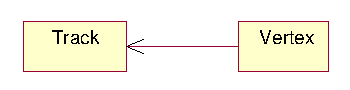
\includegraphics{umlAssociation.eps}
        \caption{Association.}
        \label{fig:umlAssociation}
    \end{center}
\end{figure}

Fig.~\ref{fig:umlAssociation} shows how we draw an association.  An
association is nothing but a line drawn between the participating
classes. In Fig.~\ref{fig:umlAssociation} the association has an
arrowhead to denote that Track does not necessarily know anything
about Vertex. This relationship will almost certainly be implemented
with a pointer of some kind.

What is the difference between an aggregation and an association?
Aggregation denotes whole/part relationships whereas associations do
not. However, there is not likely to be much difference in the way
that the two relationships are implemented.  That is, it would be very
difficult to look at the code and determine whether a particular
relationship ought to be aggregation or association.  Aggregation and
Association both correspond to the \emph{has-by-reference}
relationship.

\subsection{Dependency}

Sometimes the relationship between a two classes is very weak. They
are not implemented with member variables at all. Rather they might be
implemented as member function arguments.

Consider, for example, the fit function of a TrackFitter class.
Suppose that this function takes an argument of type CalibrartionDB
since it requires information from it (e.g. if the magnetic field was
on or off) in order to perform the fit.
\begin{figure}[htb]
    \begin{center}
        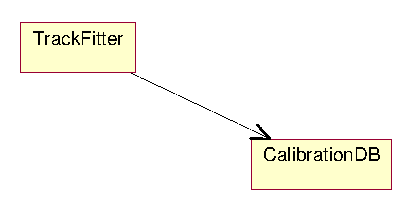
\includegraphics{umlDependency.eps}
        \caption{Dependency.}
        \label{fig:umlDependency}
    \end{center}
\end{figure}
Fig.~\ref{fig:umlDependency} shows a dashed arrow between the
TrackFitter class and the CalibrartionDB class. This is the
\emph{dependency} relationship. This is often called a \emph{using}
relationship.  This relationship simply means that TrackFitter somehow
depends upon CalibrartionDB. In C++ this almost always results in a
\#include:

{\footnotesize
\begin{verbatim}
#include "CalibrartionDB.hh"
class TrackFitter {
public:
    // ...
    void fit(CalibrartionDB &db);
private:
    // ...
};
\end{verbatim}
}%\footnotesize

%%%%%%%%%%%%%%%%%%%%%%%%%%%%%%%%%%%%%%%%%%%%%%%%%%%%%%%%%%%%%%%%%%%%
%
% The End
%
%%%%%%%%%%%%%%%%%%%%%%%%%%%%%%%%%%%%%%%%%%%%%%%%%%%%%%%%%%%%%%%%%%%%

\printindex

\end{document}
\bye
% The text following after this line is not included into the text

%
%  Template for reference section
%

%%%%%%%%%%%%%%%%%%%%%%%%%%%%%%%%%%%%%%%%%%%%%%%%%%%%%%%%%%%%%%%%%%%%
%
%    Reference: className
%
%%%%%%%%%%%%%%%%%%%%%%%%%%%%%%%%%%%%%%%%%%%%%%%%%%%%%%%%%%%%%%%%%%%%
\subsection{className}
\index{className|textbf}
\label{sec:className}
\begin{Entry}
\item[Summary]

\item[Synopsis]
    \verb+#include "className.hh"+\\
    \verb+class className;+\\

\item[Description]

\item[Persistence]
    None

\item[Related Classes]

\item[Public\\ Constructors]

\item[Public Member\\ Functions]

\item[Public Member\\ Operators]

\item[Public Functions]

\item[Public Operators]

\item[Examples]
{\footnotesize
\begin{verbatim}
//
//  What the example does
//

\end{verbatim}
}%footnotesize

\end{Entry}
